\chapter{Stanowisko demonstracyjne}
\label{cha:stanowiskodemonstracyjne}

Pierwszą częścią pracy było skompletowanie stanowiska demonstracyjnego, w skład którego wchodzą:
\begin{itemize}
	\item Kamera
	\item Platforma obliczeniowa
	\item Serwomechanizmy
	\item Sterownik serwomechanizmów
	\item Zasilanie
	\item Wskaźnik
\end{itemize}

\section{Kamera}
\label{sec:kamera}

\begin{figure}[H]
	\centering
	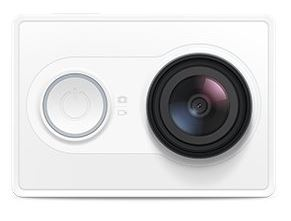
\includegraphics[width=3in]{Yi_action.jpg}
	\captionsource{Kamera Xiaomi Yi Action.}{\cite{Xiaomi}}
	\label{fig:yi_action}
\end{figure}
%TODO Może nieco mniejsze to zdjęcie... -zrobione.

Postanowiono użyć kamerę sportową Xiaomi Yi Action YDXJ01XY, widoczną na rysunku \ref{fig:yi_action}. 
Jest ona bardzo lekka i może wysyłać obraz w wybranej przez nas rozdzielczości z częstotliwością 60 Hz. 
Oprócz tego można ją przykręcić do użytych elementów połączeniowych głowicy obrotowej. 
Dane techniczne \cite{Xiaomi}:
\begin{itemize}
\item Maksymalna rozdzielczość: \(1920\)x\(1080\)
\item Waga: \(76.6\) g
\item Odporność na wstrząsy
\item Kąt nagrywania: \(155^\circ\)
\item Wymiary: \(60.4\) mm x \(42\) mm x \(21.2\) mm
\end{itemize}

\section{Platforma obliczeniowa}
\label{sec:platformaobliczeniowa}

%TODO Tu jeszcze powinien się znaleźć krótki (tak 1 - 1.5 strony) opis architektury ZYnq. Tj. schemat i omówienie poszczególnych elementów, bo potem jak Pan np. używa tego MIO to dla kogoś, kto nie jest ekspertem jest to niejasne) -zrobione. Jeśli za mało to niech mi Pan da znać.

\begin{figure}[H]
	\centering
	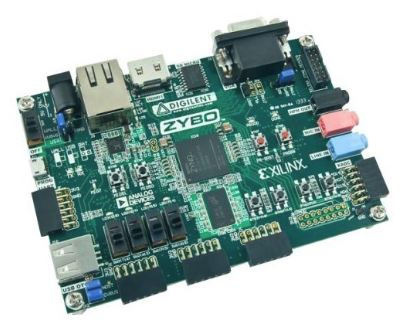
\includegraphics[width=4in]{zybo.jpg}
	\captionsource{Karta ewaluacyjna ZYBO Zynq-7000.}{\cite{Xi}}
	\label{fig:zybo}
\end{figure}
%TODO Tu jakaś za duża ta biała ramka na około ... -zrobione.

Zdecydowano, że platformę obliczeniową stanowić będzie karta ewaluacyjna ZYBO. %TODO płytka -> karta uruchomieniowa/ewaluacyjna -zrobione.
Przedstawiona została na rysunku \ref{fig:zybo}.
Jest to bogato wyposażone urządzenie zawierające układ programowalny z rodziny Xilinx Zynq-7000. %TODO narzędzie ? -zmieniono na urządzenie.
Układ ten oparty jest na architekturze Xilinx All Programable System-on-Chip, w której zintegrowany został dwurdzeniowy procesor ARM Cortex-A9 i układ programowalny FPGA z serii Xilinx 7.

\begin{figure}[h]
	\centering
	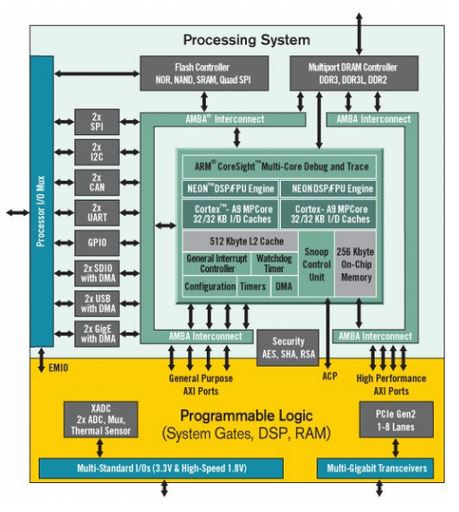
\includegraphics[width=4in]{zybo_scheme.jpg}
	\captionsource{Schemat architektury Zynq AP SoC.}{\cite{Xi}}
	\label{fig:zybo_scheme}
\end{figure}

Na rysunku \ref{fig:zybo_scheme} przedstawiono schemat architektury Zynq AP Soc, z procesorem(PS) zaznaczonym kolorem zielonym i logiką rekonfigurowalną(PL) żółtym. FPGA jest konfigurowane bezpośrednio przez procesor lub przez port JTAG. PS składa się z wielu komponentów, wliczając w to APU(Application Processing Unit, składające się z dwóch rdzenie Cortex-A9). Wyjścia układów peryferyjnych PS mogą być podłączone do MIO(Multiplexed Input/Output), lub EMIO. MIO są wyprowadzone do pinów układu Zynq, natomiast EMIO łączą PS z PL. Oprócz EMIO do łączenia części rekonfigurowanej z procesorem w układzie Zynq służą elementy przemysłowego standardu interfejsów AXI, które zapewniają dużą przepustowość i niską latencję połączeń\cite{Zynq}. Umożliwiają m.in. przesyłanie danych z PL do PS bez użycia procesora, z użyciem DMA(Direct Memory Access). Rozwiązanie to jest bardzo korzystne, gdy przesłać musimy dużą ilość danych, np. kompletną ramkę obrazu.

Karta ewaluacyjna zawiera m.in. port HDMI potrzebny do odbierania obrazu z kamery oraz port VGA, który umożliwia nam wysyłanie obrazu do monitora \cite{Xi}.
W układzie programowalnym zaimplementowany zostanie tor wizyjny przetwarzający potokowo dane przesyłane z kamery oraz wyznaczający położenie obiektu w danej ramce.
Oprócz tego musi on komunikować się ze sterownikiem serwomechanizmów w celu pozycjonowania głowicy w wyznaczonym punkcie oraz z komputerem klasy PC, aby otrzymywać parametry pracy oraz ustawiać początkową pozycję głowicy.

\section{Serwomechanizmy}
\label{sec:serwomechanizmy}

%TODO Przydała by się referencja na podstawie której te wady/zalety są zawsawione -zmienione. \cite{Salt}

Ruchomą głowicę postanowiono skonstruować wykorzystując serwomechanizmy dostępne na rynku. 
Przy wyborze brano pod uwagę serwomotory analogowe, cyfrowe oraz smart.
%TODO powt. x3 serwo... jakoś to zgrabniej proszę opisać. -przepisano, zmieniono na serwomotor.

\subsection{Serwomechanizm analogowy}
Urządzenie to jest sterowane impulsami przekazywanymi z częstotliwością 50 Hz.
Podawanie impulsów z większą częstotliwością może doprowadzić do uszkodzenia urządzenia.
%TODO powt. podawanie... -zmieniono na przekazywanie.
W zależności od czasu trwania impulsu serwomotor ustawia się w odpowiedniej pozycji i ją utrzymuje. 
Kontrola położenia odbywa się za pomocą potencjometru sprzężonego z kołem zębatym. 
Serwomechanizmy tego typu nie reagują szybko i nie generują wystarczającego momentu kiedy zadane zostają małe przesunięcia \cite{Salt}.
%TODO produkują -> złe słowo !!! -zmienono na generują.

\subsection{Serwomechanizm cyfrowy}

Jest on, podobnie jak serwomotor analogowy, sterowany impulsami. 
Podawać można je jednak z maksymalną częstotliwością powyżej 300 Hz. 
W porównaniu do serwomechanizmu analogowego przyspiesza ono szybciej i generuje stabilniejszy moment obrotowy. 
%TODO produkuje -zmieniono na generuje.
Reagują również lepiej na polecenia małych zmian pozycji. 
Z drugiej strony potrzebują one dużo większej mocy \cite{Salt}.
Prąd, który pobierają w trakcie pracy, może sięgać kilku amperów.

\subsection{Serwomechanizm smart}
Główną różnicą pomiędzy serwomechanizmami standardowymi, a smart, jest sposób komunikacji w celu podania wartości zadanej położenia.
Zamiast impulsów o różnej szerokości wykorzystuje się komunikację szeregową.
Ich obsługa jest więc bardziej skomplikowana. Najpopularniejszymi protokołami są TTL Half-Duplex, TTL Full-Duplex i RS-485.
Za pomocą komunikacji tego typu możliwa jest konfiguracja znacznie większej ilości parametrów pracy, niż tylko pozycja zadana.
Można zmieniać nastawy regulatora PID, maksymalną prędkość kątową lub maksymalny moment. %TODO powt. zmieniać. -zmieniono na konfigurować.
W przeciwieństwie do serwomechanizmów klasycznych, możliwe jest również odczytywanie aktualnej pozycji serwomechanizmu.
Minusem tych urządzeń jest ich cena oraz dostępność.
Są one kilka razy droższe od cyfrowych serwomotorów o podobnych parametrach.

\paragraph*{}

\begin{figure}[h]
	\centering
	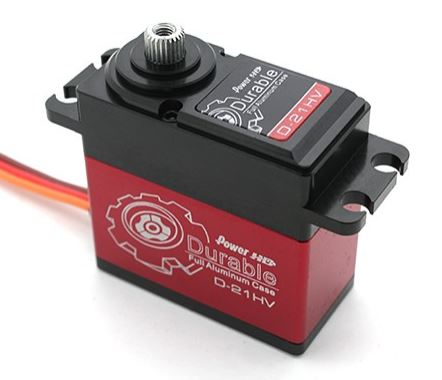
\includegraphics[width=3in]{Pololu.jpg}
	\captionsource{Serwomechanizm cyfrowy PowerHD D-21HV.}{\cite{Pololu}}
	\label{fig:pololu}
\end{figure}

Ostatecznie postanowiono użyć dwóch serwomechanizmów cyfrowych PowerHD D-21HV.
Przedstawiono je na rysunku \ref{fig:pololu}.
Są to urządzenia typu standard o dużym momencie obrotowym i wysokiej maksymalnej prędkości obrotowej. 
Wyposażone są one w łożyska kulkowe oraz tytanowe tryby w celu zwiększenia  wytrzymałości. 
Specyfikacja techniczna \cite{Pololu}:
\begin{itemize}
\item Napięcie zasilania: \(6.0-7.4\) V
\item Zakres ruchu: \(155^\circ\)
\item Masa: \(75\) g
\item Moment: \(21\) kg\(\cdot\)cm dla napięcie \(7.4\) V
\item Prędkość: \(0.12\)s/\(60^\circ\) dla napięcia \(7.4\) V
\end{itemize}
Urządzenia te mogą pobierać impulsowy prąd o wartości nawet powyżej 3 A.
Sterowane są za pomocą impulsów podawanych z częstotliwością 333 Hz.
Pozycja neutralna zadana zostaje poprzez podanie impulsu o czasie trwania \(1500 \mu\)s. %TODO naturalną, czy neutralną ? -zmieniono.
Serwa zostały połączone w głowicę za pomocą metalowych uchwytów dedykowanych do łączenia serwomechanizmów typu standard w konfigurację PT.
Konfiguracja PT (Pan-Tilt) jest to takie połączenie urządzeń obrotowych, że jedno odpowiada za nachylenie, a drugie za obrót.
%TODO objaćnić to PT -zrobione.
%TODO Też może nico mniejsze to zdjęcie serwomechanizmu -zmieniono.

\section{Sterownik serwomechanizmów}
\label{sec:sterownik}
%TODO tutat trzeba zwrócić uwagę, czy się za dużo pustego miejsca nie robi !! -zrobiłem, ale musiałem przenieść orazek do środka tekstu, zamiast na początku.

\begin{figure}[h]
	\centering
	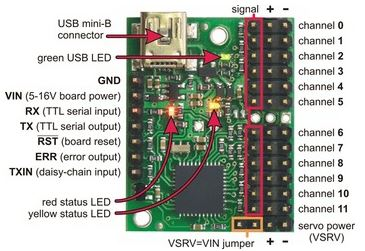
\includegraphics[width=4in]{maestro.jpg}
	\captionsource{Sterownik serwomechanizmów Pololu Mini Maestro.}{\cite{MM}}
	\label{fig:maestro}
\end{figure}

Do sterowania serwomechanizmami postanowiono użyć gotowego sterownika produkowanego przez firmę Pololu, widocznego na rysunku \ref{fig:maestro}.
12-kanałowy sterownik Mini Maestro pozwala na równoczesną obsługę obu serwomechanizmów. 
Oprócz podawania wartości zadanej w postaci impulsów pozwala on również na zmianę ustawianie maksymalnej prędkości obrotowej i maksymalnego momentu obrotowego. 
Dzięki temu można dużo lepiej kontrolować urządzenia wykonawcze i zapewnić bardziej ciągły ruch głowicy. 
Komunikacja ze sterownikiem odbywa się za pośrednictwem interfejsu szeregowego UART z prędkością 115200 bitów na sekundę.

\section{Zasilanie}
\label{sec:zasilanie}

\begin{figure}[H]
	\centering
	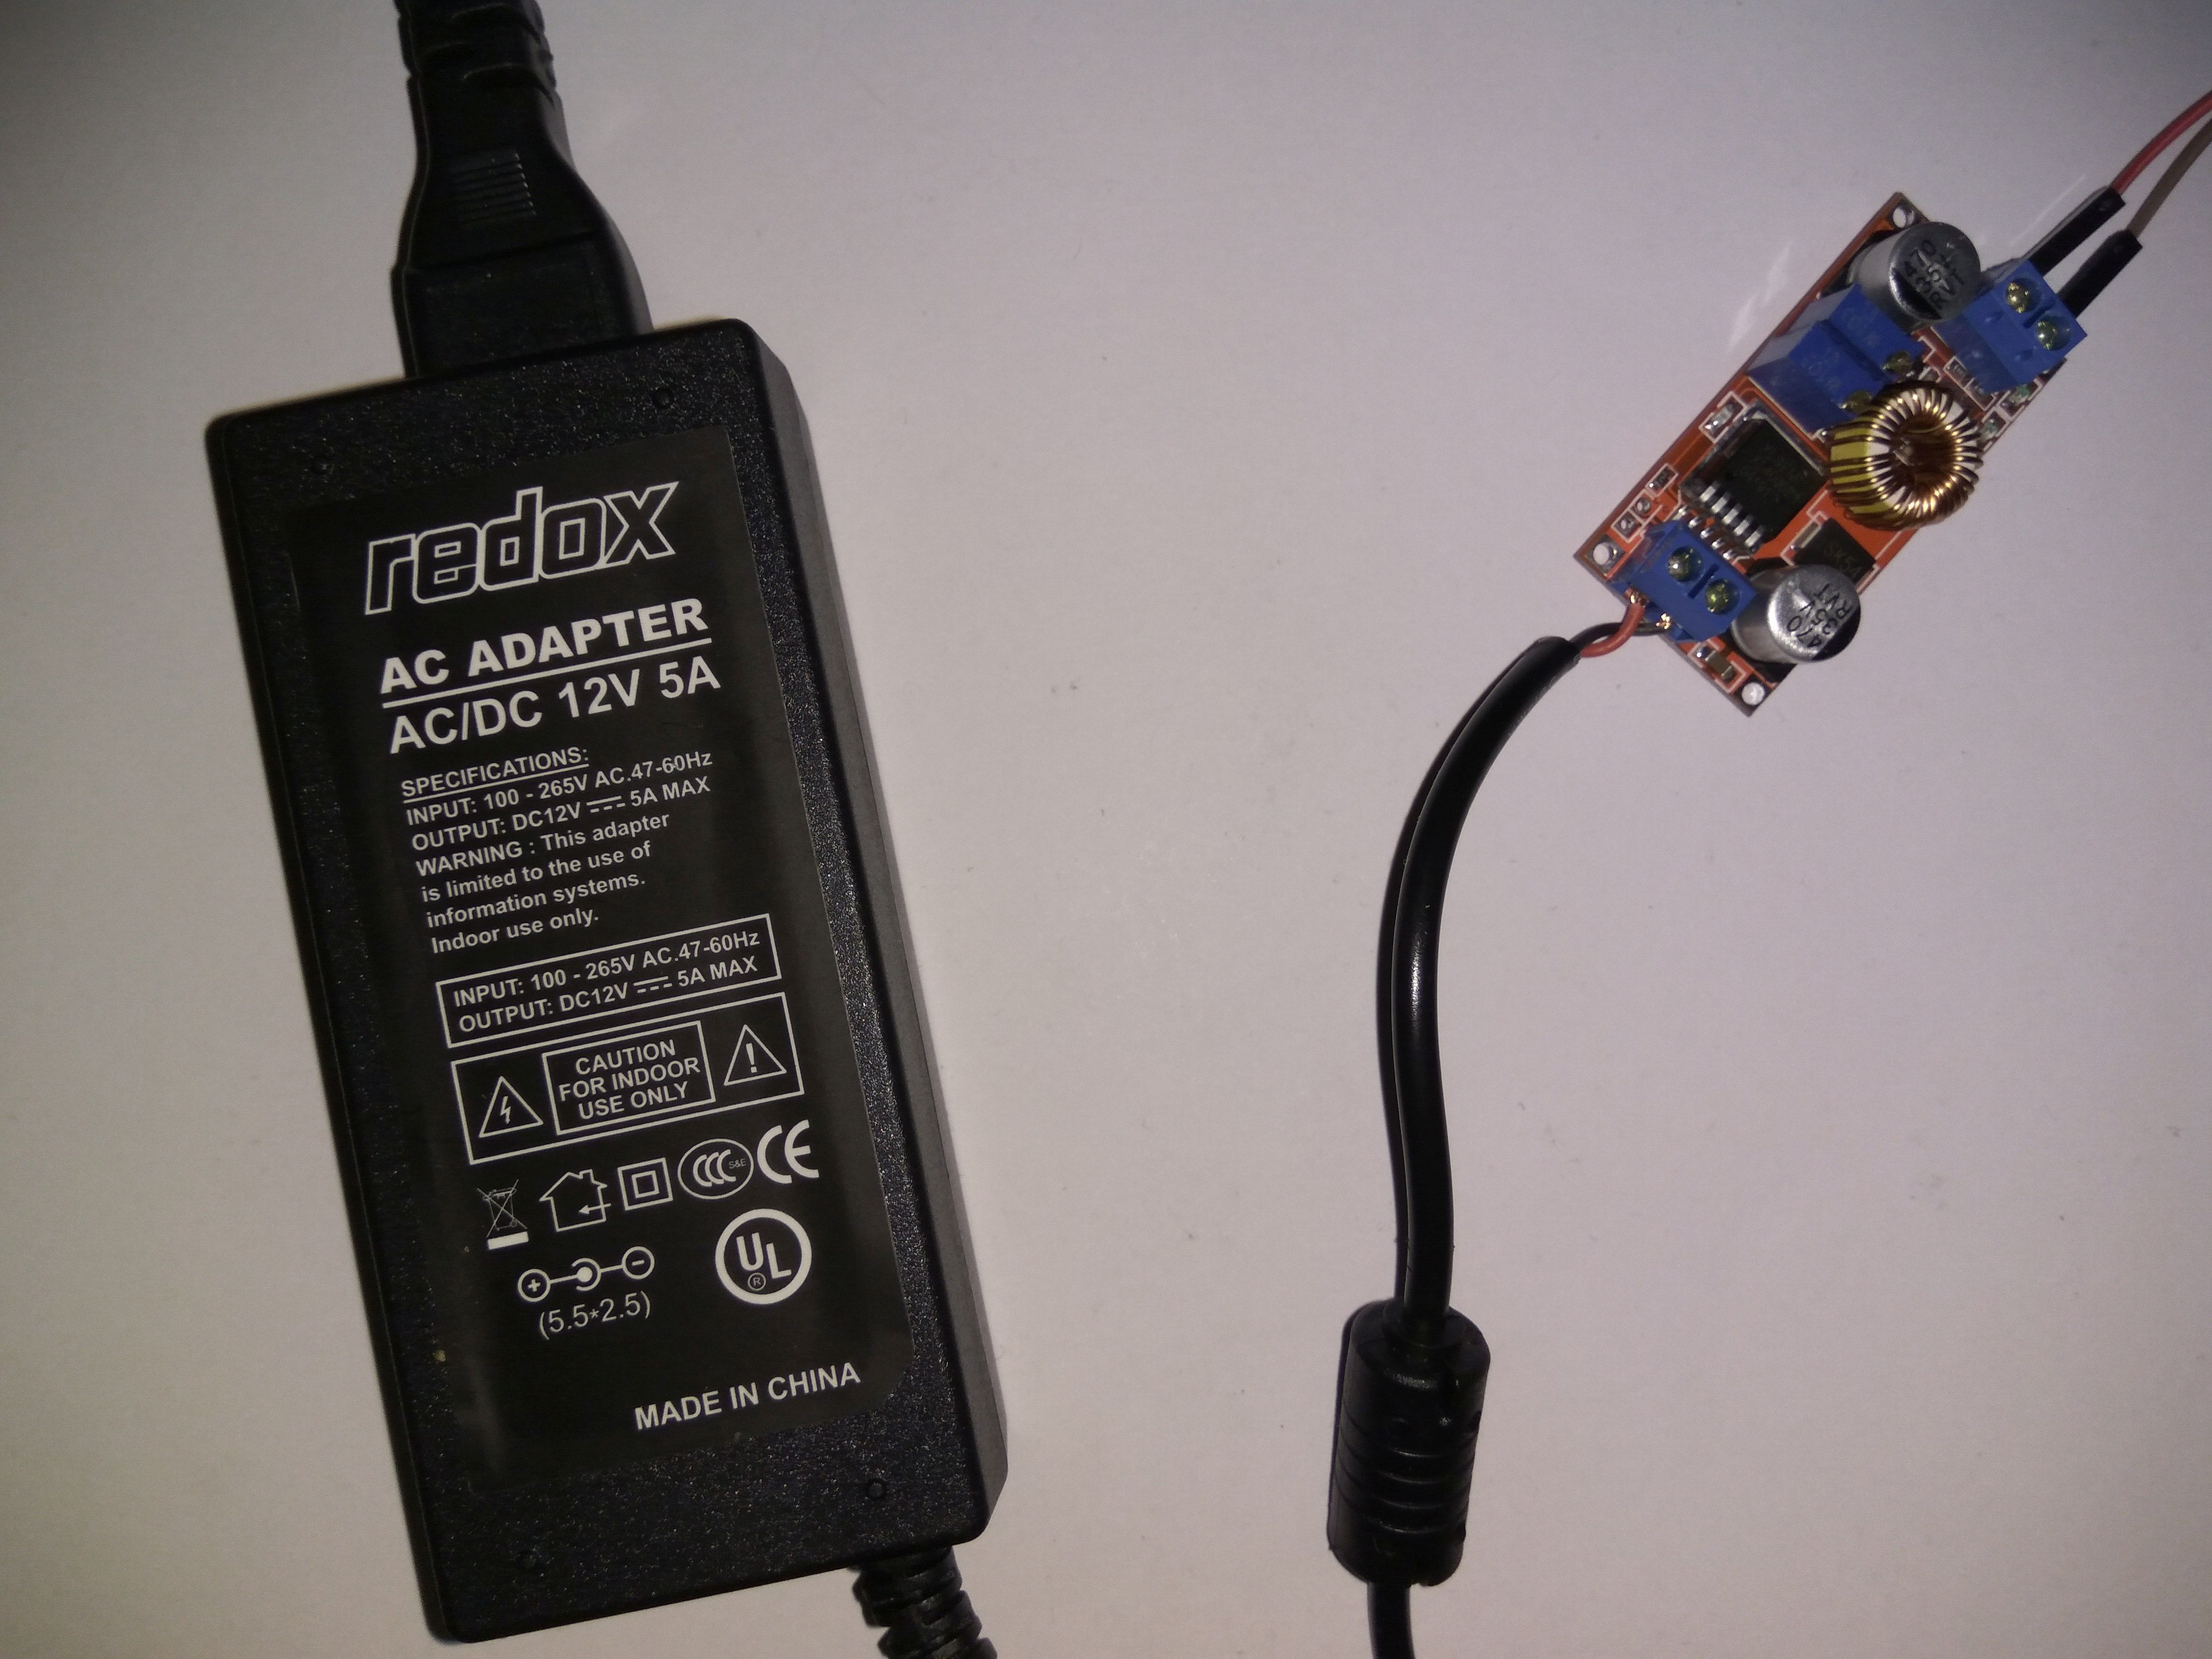
\includegraphics[width=4in]{zasilanie.jpg}
	\caption{Układ zasilający serwomechanizmy.}
	\label{fig:zasilanie}
\end{figure}

Do zasilania głowicy użyty został zasilacz impulsowy Redox, który na wyjściu daje napięcie 12 V i maksymalny prąd 5 A. Jako, że serwomechanizmy potrzebują napięcia 7.4 V użyta została przetwornica \textit{step-down} XL4005E1 o regulowanym napięciu wyjściowym. Maksymalny prąd wyjściowy użytej przetwornicy wynosi 5 A.
Jest to wartość wystarczająca do zasilenia użytych serwomechanizmów.
Elementy te zostały przedstawione na rysunku \ref{fig:zasilanie}.

\section{Wskaźnik}
\label{sec:wskaznik}

Postanowiono użyć zwykłego wskaźnika laserowego do wskazywania miejsca, w stronę którego zwrócona jest głowica. Należy zauważyć, że miejsce nie jest wskazane dokładnie, gdyż wskaźnik jest przesunięty względem kamery oraz nie jest idealnie do niej równoległy.

\begin{figure}[h]
	\centering
	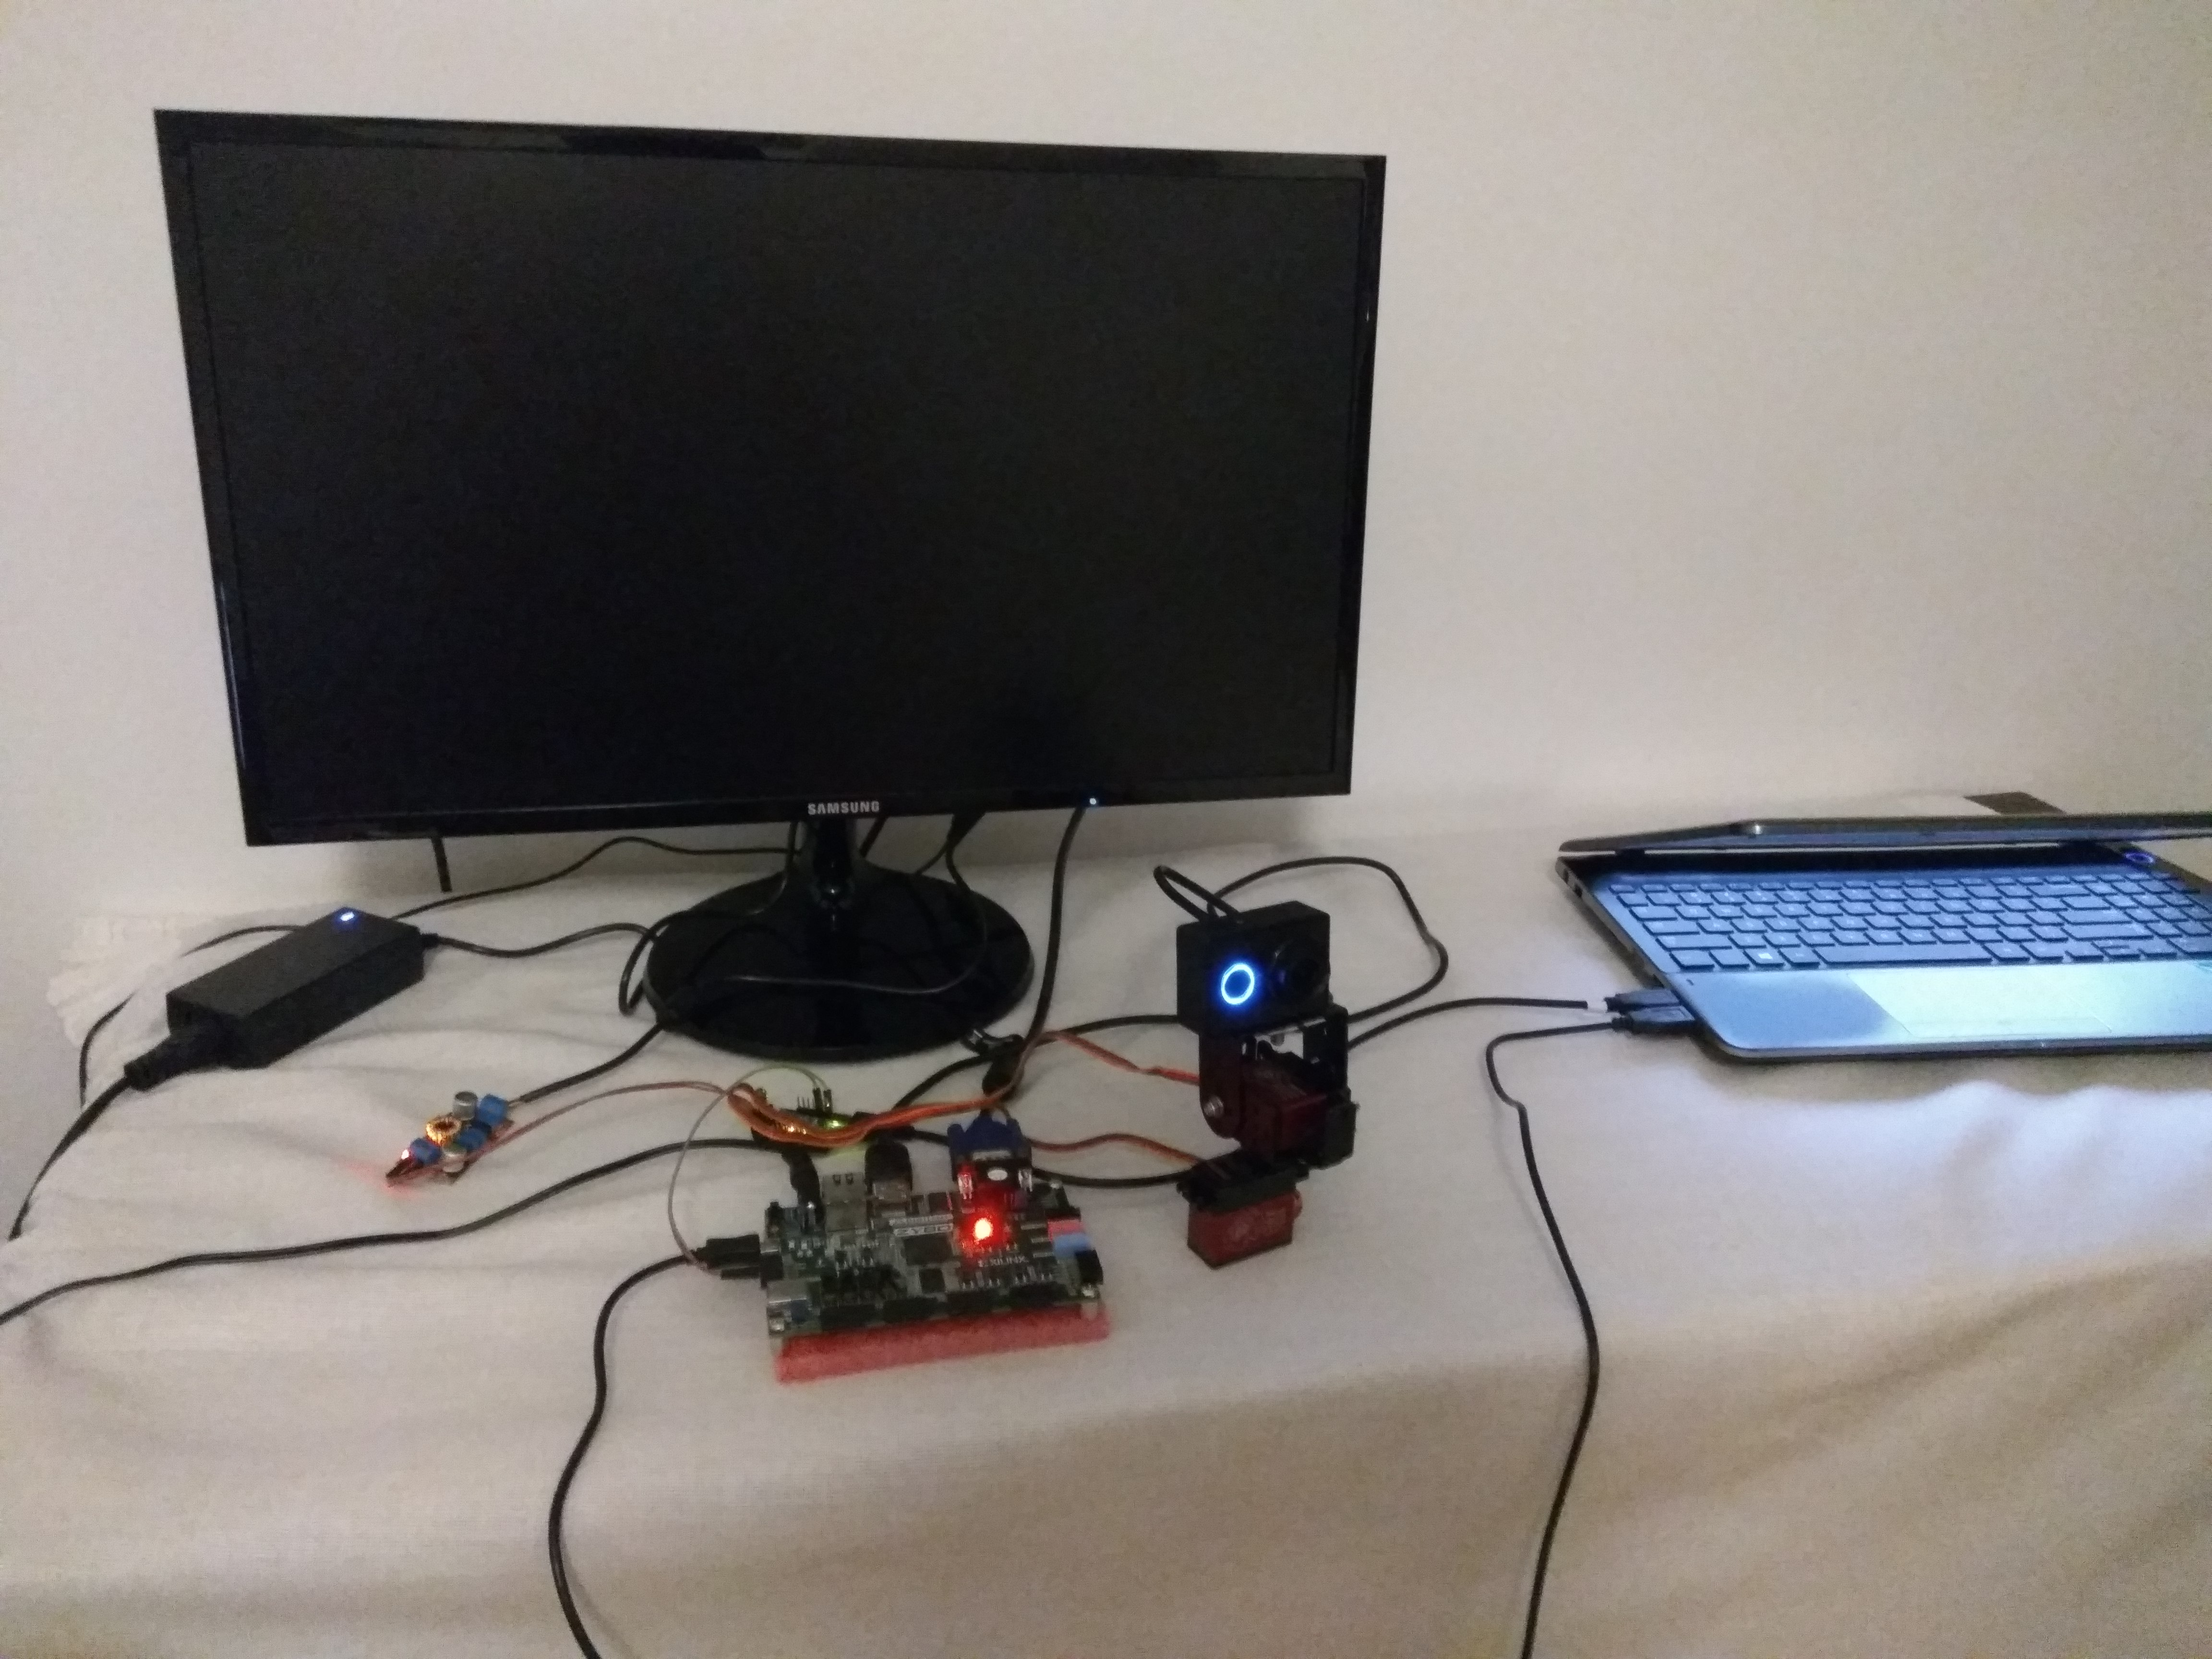
\includegraphics[width=4in]{kompletne_stanowisko.jpg}
	\caption{Zbudowane stanowisko.}
	\label{fig:kompletne_stanowisko}
\end{figure}

Rysunek \ref{fig:kompletne_stanowisko} przedstawia kompletne stanowisko, na którym wykonywany był projekt. Oprócz opisanych elementów na zdjęciu widoczny jest monitor, który służył do wizualizacji wyników działania systemu. Sterownik serwomechanizmów jest zasilany z portu USB komputera PC. Z komputerem jest również połączona karta ewaluacyjna ZYBO, w celu programowania przez JTAG oraz komunikacji.
%TODO Tu aż się prosi dać zdjęcie całego stanowiska !! -zrobione.